\documentclass[11pt]{article}

\usepackage{float}
\usepackage{hyperref}
\usepackage{fullpage}
\usepackage{verbatim}
\usepackage{moreverb}
\usepackage{graphicx}
\usepackage{parskip}
\usepackage{amsmath}
\usepackage{etoolbox}
\usepackage[toc,page]{appendix}
\graphicspath{{images/}}
\usepackage{gensymb}

\usepackage{minted}
\let\verbatiminput=\verbatimtabinput
\def\verbatimtabsize{4\relax}

\begin{document}
\title{EE 241B HW4 Writeup}

\author{Vighnesh Iyer}
\date{}
\maketitle

\tableofcontents

\section{Delay Replicas}
\begin{quote}
	Your design has a critical path of 20 FO4 inverter delays at the nominal supply voltage. Your friend has suggested to design a replica circuit consisting of N FO1 inverters (where N is approximately 40.
\end{quote}

\subsection{Replica Design}
\begin{quote}
	Design the actual replica made of N-1 identical stages with the Nth stage having an increased fanout to match the actual critical path. What is the fanout of the Nth stage?
\end{quote}

We begin by calculating the critical path delay in terms of minimally sized inverter delays $t_{inv}$ using the method of logical effort. We first define all the variables that are used for logical effort delay calculations.

\begin{align}
	f &= \text{ fanout of single stage} = C_{out} / C_{in} \nonumber \\
	F &= \text { total fanout} = C_{L,total} / C_{in} \nonumber \\
	\text{EF} &= \text { effective fanout} = \text{LE} f \nonumber \\
	p &= \text{ intrinsic delay (ratio of PMOS to NMOS capacitance)}; p_{inv} = \gamma \nonumber \\
	\text{LE} &= \text { logical effort} = (R_{eq,gate} C_{in,gate}) / (R_{eq,inv} C_{in,inv}); LE_{inv} = 1 \nonumber \\
	\text{b} &= \text{ branching factor} = \frac{C_{L,on-path} + C_{L,off-path}}{C_{L,on-path}} \nonumber \\
	\text{PE} &= \text{ path effort} = (\prod \text{LE}) (\prod b) F \nonumber \\
	t_{p,gate} &= t_{inv}(p + \text{LE}f) = t_{inv}(p + \text{EF}) \nonumber
\end{align}

Now we calculate the critical path delay.

\begin{align}
	t_{delay,inv} &= t_{inv}(p_{inv} + \text{LE} f) \nonumber \\
	t_{delay,inv} &= t_{inv}(\gamma + 4) \nonumber \\
	t_{delay,crit-path} &= t_{delay,inv}  \cdot N_{stages} = 20 \cdot t_{inv}(\gamma + 4) \nonumber
\end{align}

Let's now consider the path that consists of 39 FO1 inverters and 1 larger inverter. We can break this path's delay into 2 sub-delays.

\begin{align}
	t_{delay,replica1} &= 39 \cdot t_{inv}(\gamma + 1) \nonumber \\
	t_{delay,replaca2} &= t_{inv}(\gamma + f_{last,stage}) \nonumber \\
	t_{delay,replica} &= 39 t_{inv}(\gamma + 1) + t_{inv}(\gamma + f_{last,stage}) \nonumber \\
	\text{Set } t_{delay,replica} &= t_{delay,crit-path} \nonumber 
\end{align}

Performing calculations, and assuming $\gamma = 1$ for a modern process, we get $f_{last,stage}$ = 21, and an approximate area reduction for the replica from 80 to 60.

\subsection{Replica Tracking Across Different Gates}
\begin{quote}
	There are three nearly identical critical paths in the circuit, one consisting of 20 FO4 inverters, one consisting of all NAND2s and one consisting of all NOR2s. Simulate tracking of the replica from part a) from the nominal down to 0.5V with 50 mV steps.
\end{quote}

I performed a SPICE simulation with 4 logic paths (replica, inverter chain, NAND2 chain, NOR2 chain). I created the inverter chain with 50 FO4 inverters to 'match' the delay of 20 FO4 inverters to avoid having to upsize every inverter along the chain. The NAND2 and NOR2 chains were created with 33 and 11 gates respectively to match the delay of the inverter chain (the number of gates was determined from simulation). The replica was designed exactly as described in part a).

I wrote a Python script to generate the SPICE netlist to simulate. It is attached in the appendix. The results are:

\begin{figure}[H]
	\centerline{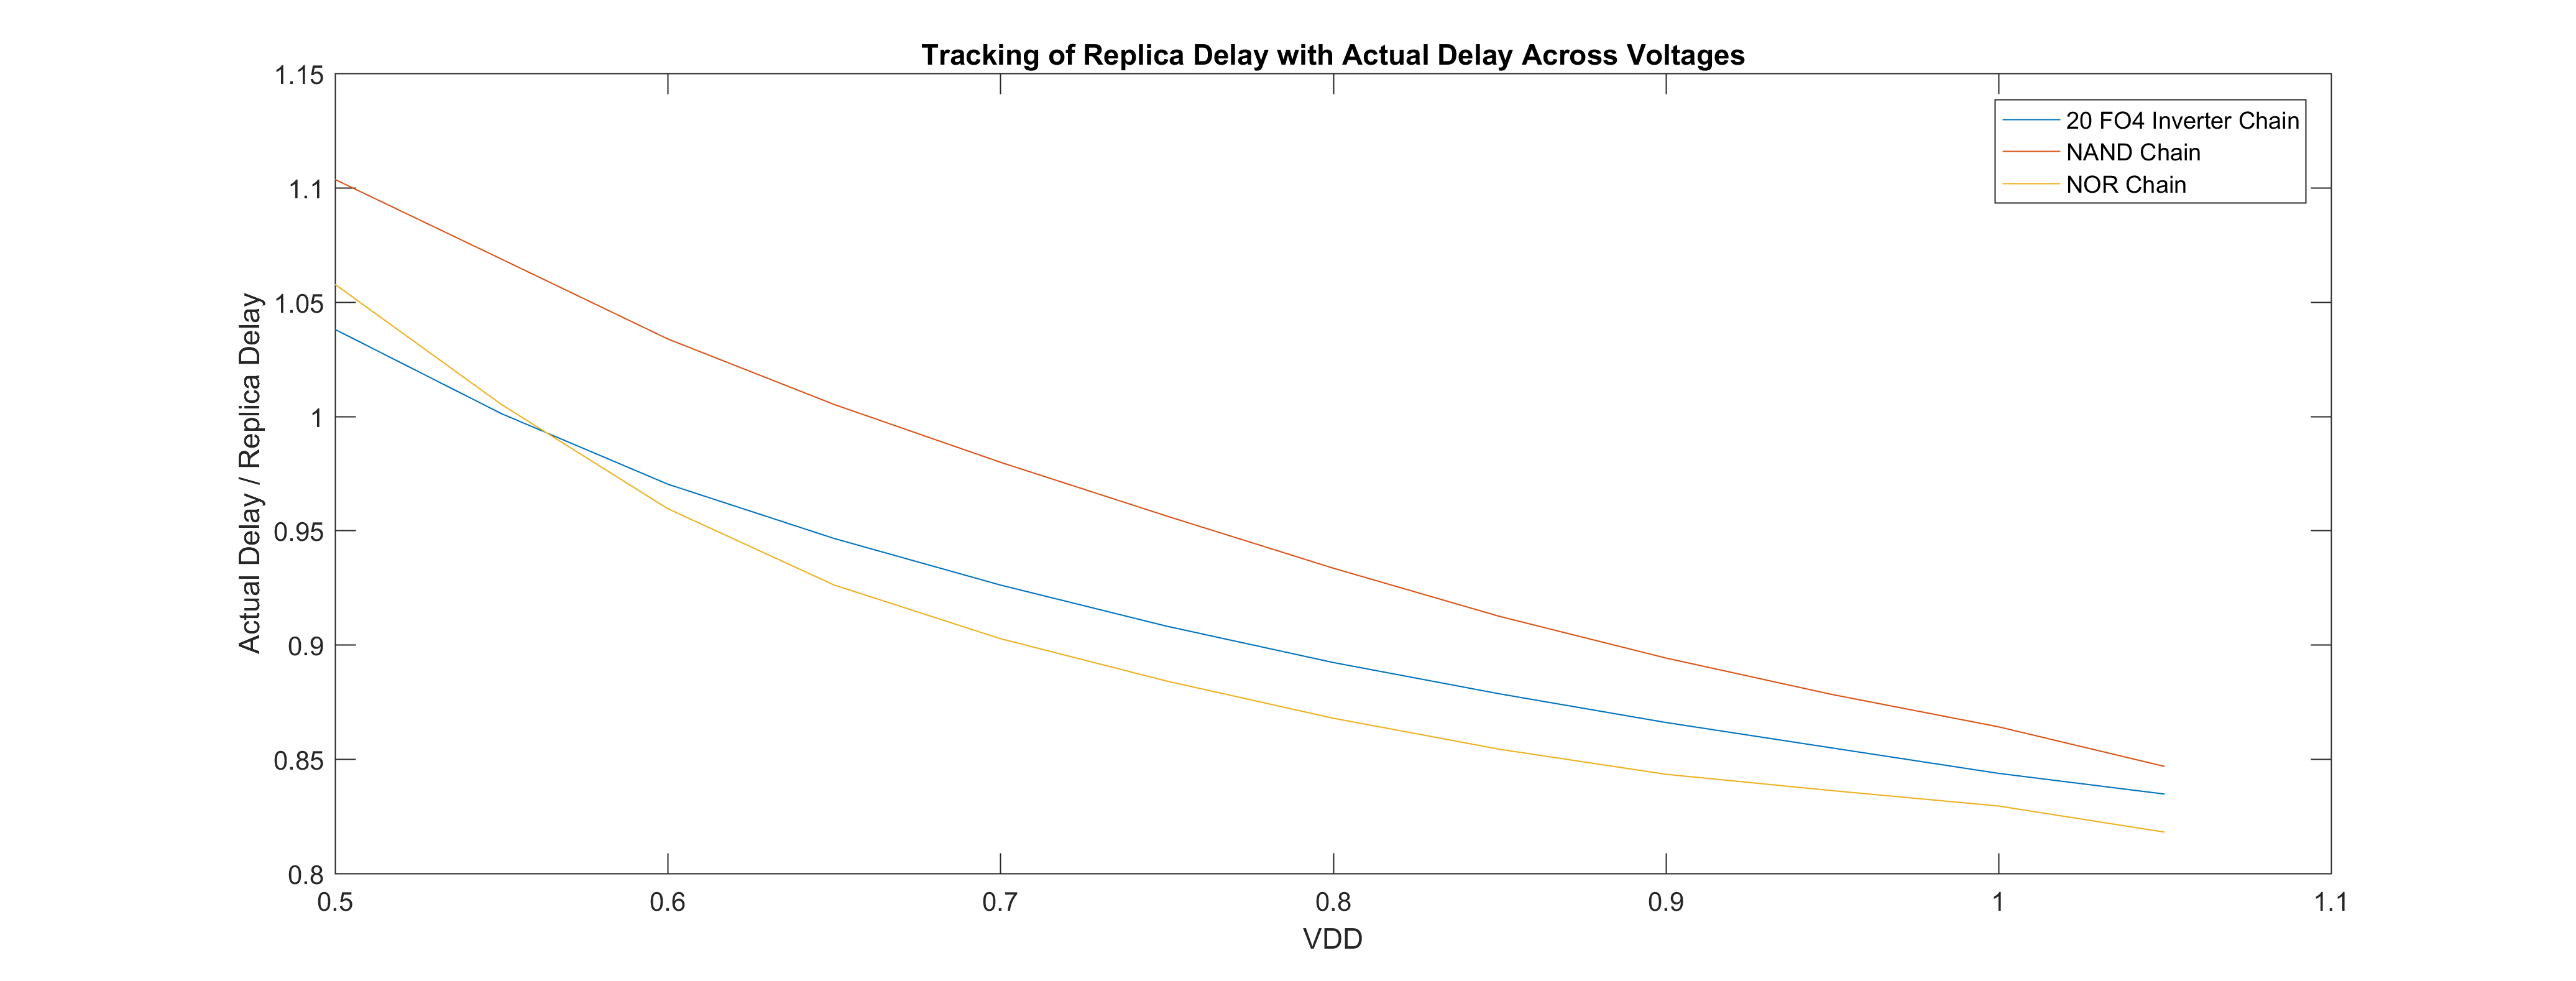
\includegraphics[width=\textwidth]{images/replica_tracking.png}}
\end{figure}

It can be seen that at the nominal supply voltage all 3 logic paths start at around the same place and the replica overestimates their delay to keep the timing constraints met. However as voltage scales down, the NOR and inverter chain is tracked at least to a proportional constant, but the NAND chain deviates non-linearly. In all cases, at low voltages, the replica fails to accurately estimate the actual delays and timing failure can happen.

\subsection{Replica Redesign}
\begin{quote}
	How would you design the replica to accurately track these critical paths across the supply voltage range?
\end{quote}

We could design a configurable delay replica which could have different circuits multiplexed in at lower voltages. Based on the supply voltage, the delay chain would involve a different set of gates that would better track the increased delay that would result. For instance at lower voltages, a replica delay line that was based on a chain of NAND2 gates would provide additional safety margin for timing.

\section{Power-performance Tradeoffs}

\subsection{Energy/Delay Sensitivity}
\begin{quote}
	Using the alpha-power law model, derive the analytical expression for the energy/delay sensitivity of a design to scaling of supply voltage. Evaluate this expression at the nominal supply voltage, using the results from Homework 1 ($K = 0.001, \alpha = 1.5, V_{th} = 0.45 \text{V for NMOS}$)
\end{quote}

We can model the switching NMOS transistor as a current source (dis)charging its self-capacitance and load capacitance which we lump together as $C$.

\begin{align}
	I_D &= K (V_{GS} - V_{th})^\alpha \propto t_{delay} \nonumber \\
	V_{GS} &= V_{DD} \text{ assuming instant switching} \nonumber \\
	\text{for NMOS's capacitor } V(t) &= \frac{Q(t)}{C} = \frac{1}{C}\int_{0}^{t}I(t) dt = \frac{1}{C}\int_{0}^{t} K (V_{DD} - V_{th})^\alpha dt \nonumber \\
	&= \frac{1}{C} K (V_{DD} - V_{th})^\alpha t = V_{DD} \nonumber \\
	t_{delay} &= \frac{V_{DD} K C}{(V_{DD} - V_{th})^\alpha} \nonumber \\
	E_{gate} &= C V_{DD}^2 \nonumber
\end{align}

To get sensitivities to $V_{DD}$ take derivatives with respect to $V_{DD}$.

\begin{align}
	\frac{\partial t}{\partial V_{DD}} = K C \frac{(\alpha - 1)V_{DD} + V_{th}}{-(V_{DD} - V_{th})^{\alpha + 1}} \nonumber \\
	\frac{\partial E}{\partial V_{DD}} = 2 C V_{DD} \nonumber \\
	\frac{\partial E}{\partial V_{DD}} \bigg/ \frac{\partial t}{\partial V_{DD}} = \frac{2 V_{DD}}{K} \cdot \frac{-(V_{DD} - V_{th})^{\alpha+1}}{(\alpha - 1)V_{DD} + V_{th}} \nonumber 
\end{align}

In this calculation we don't factor leakage energy into the gate's energy since we are concerned with energy vs delay tradeoffs, which involve switching energy.

\subsection{Energy/Delay Sensitivity to Logic Depth}
\begin{quote}
	What is the energy/delay sensitivity of a design to the logic depth? You can define the logic depth as a number of FO4 inverters that fit into one clock period.
\end{quote}

Lets say that there are $N$ inverter stages in a logic path. Then, the delay is linearly proportional to $N$ because the fanout of each stage is fixed and each inverter is sized to have the same pull-up/pull-down strength as the minimally sized inverter.

\begin{align}
	t_{delay,path} \propto N \cdot t_{delay} = \frac{V_{DD} K C N}{(V_{DD} - V_{th})^\alpha} \nonumber 
\end{align}

However, the energy is dependent on the total capacitance of each inverter along the path:

\begin{align}
	E_{path} = V_{DD}^2 \cdot (C + \sum_{x = 1}^{N}(C \cdot 4^x)) = V_{DD}^2 (C + \frac{4}{3} C (4^N - 1)) \nonumber
\end{align}

Taking derivatives wrt $N$:

\begin{align*}
	\frac{\partial t_{delay,path}}{\partial N} = \frac{V_{DD} K C}{(V_{DD} - V_{th})^\alpha} \\
	\frac{\partial E_{path}}{\partial N} = \frac{1}{3} V_{DD}^2 \cdot C \cdot 4^{N+1} \ln(4) \\
	\frac{\partial E_{path}}{\partial N} \bigg/ \frac{\partial t_{delay,path}}{\partial N} = \frac{V_{DD} 4^{N+1} \ln(4) (V_{DD} - V_{th})^\alpha}{3K}
\end{align*}

So it can be concluded that the energy is much more sensitive to changes in the logic depth than the delay as would be expected.

\section{Subthreshold Design}
\subsection{Subthrehold Dependence on Supply Voltage}
\begin{quote}
	From the lecture notes, it appears that for a design operating in subthreshold, the minimum energy point of a design does not depend on the threshold voltage, and only depends on the supply. Can you explain why (very briefly)?
\end{quote}

To be brief, the leakage current becomes active switching current when operating in subthreshold. Then the leakage energy becomes dependent not only on the leakage current but the delay, which is affected in the opposite way by the threshold voltage. These two terms 'cancel out' and the threshold voltage doesn't make a difference in the minimum energy point.

\subsection{Threshold Voltage Importance}
\begin{quote}
	If it doesn't matter for the energy consumption, why is it important to control the transistor threshold voltage in subthreshold design?
\end{quote}

Delay is very sensitive to the threshold voltage when $V_{DD}$ is near the threshold voltage. So even though energy savings don't depend on the threshold, the circuit timing and retention-ability of static circuits depend greatly on the threshold voltage.

\section{Stack Forcing}
\begin{quote}
	What is the sensitivity in the energy-delay space of stack forcing technique, applied to every inverter in an optimally sized (for minimum delay) inverter chain of length 6? The input capacitance is 1fF, and the initial leakage is 30\% of the total energy dissipated by the inverters. Assume that the $C_{d} = C_{g} = 2$ fF$/\mu$, and a linear delay model is used. $V_{DD}$ = 1V and the stack of 2 reduces the leakage by a factor of 10.
\end{quote}

Taking the original 6 inverter chain, we want to find its delay and energy consumption. The fanout of each inverter ought to be equal to minimize delay, and we can simply assume a fanout of 4 for each inverter (although this would be process dependent and based on $\gamma$; we assume $\gamma = 1$ in this problem just to make calculations easy). We also assume that the PMOS mobility is half that of the NMOS.

The minimally sized inverter is to have 1fF of input capacitance so it stands that the NMOS is 1/6 $\mu$ and the PMOS is 2/6 $\mu$ in width.

\begin{align}
	t_{inv,minimal} &= \ln(2) R \text{ 1 fF} \nonumber \\
	t_{inv,FO4} &= t_{inv,minimal} (\gamma + f) = t_{inv,minimal} \cdot 5 = \ln(2) R \text{ 5 fF} \nonumber \\
	t_{path} &= 6 \cdot t_{inv,FO4} = \ln(2) R \text{ 30 fF} \nonumber \\
	E_{path,dyn} &= C_{total} V_{DD}^2 = (1 + \sum_{x=1}^{5}2 \cdot 4^x + 4096) 1^2 = (1 + 2728 + 4096) = 6825 \text{ fJ} \nonumber \\
	E_{path,leak} &= E_{path,dyn} \cdot \frac{0.3}{0.7} = 2925 \text{ fJ}\nonumber \\
	E_{path,total} &= 9570 \text{ fJ} \nonumber
\end{align}

Now we assume that stack forcing is on and that every inverter is made up of 2 stacked NMOSs and 2 stacked PMOSs with their gates tied together as usual. We also assume that the widths of the NMOS and PMOS transistors are cut in half to maintain the same input capacitance and fanout. This results in an effective switching resistance that is 4x greater than the un-stacked inverter due to the halving of widths and the stacking (assuming linear delay model). The self-loading capacitance of each inverter goes down by 2x assuming we neglect the stack node capacitance.

\begin{align}
	%t_{inv,minimal} &= \ln(2) 4 R \text{ 0.5 fF} \nonumber \\
	t_{inv,FO4} &= \ln(2) 4R \text{ 4.5 fF} \nonumber \\
	t_{path} &= 6 \cdot \ln(2) 4R \text{ 4.5 fF} \nonumber \\
	E_{path,dyn} &= (.5 + \sum_{x=1}^{5}(4^x + 4^x/2) + 4096) 1^2 = 6142.5 \text{ fJ} \nonumber \\
	E_{path,leak} &= E_{path,leak,orig} / 10 = 292.5 \text{ fJ} \nonumber \\
	E_{path,total} &= 6435 \text{ fJ} \nonumber
\end{align}

We can now calculate the sensitivity:

\begin{align}
	\frac{\partial E}{\partial \text{stack}} \bigg/ \frac{\partial t}{\partial \text{stack}} = \frac{\Delta E}{\Delta t} &= \frac{9570 - 6435 \text{ fJ}}{\ln(2) R \text{ 30 fF} - \ln(2) R \text{ 108 fF}} \nonumber \\
	&= \frac{3135 \text{ fJ}}{-R \cdot 54 \text{ fF}} \nonumber
\end{align}

where $R$ can be approximated through simulating the switching current characteristic of an inverter.

\newpage
\appendix
\section{Python SPICE Generation Script}
\begin{minted}[breaklines]{python}
preamble_string = """Simulating VDD scaling and replica delay

.lib '/home/ff/ee241/synopsys-32nm/hspice/saed32nm.lib' TT

* Parameters and supplies
.param VDD_val=1.05
vdd vdd gnd VDD_val
vin vin gnd pwl(0 0 1n 0 1.1n VDD_val)

* Library standard cells that are used in this testbench

*  Library name: saed32nm_rvt
*  Cell name: INVX0_RVT
*  View name: schematic
.subckt invx0_rvt a vdd vss y
xmp y a vdd vdd p105 m=1 w=520e-9 l=30e-9 ad=10.5e-15 as=10.5e-15 pd=310e-9 ps=310e-9
xmn y a vss vss n105 m=1 w=270e-9 l=30e-9 ad=10.5e-15 as=10.5e-15 pd=310e-9 ps=310e-9
.ends

*  Library name: saed32nm_rvt
*  Cell name: INVX32_RVT
*  View name: schematic
.subckt invx32_rvt a vdd vss y
xmp y a vdd vdd p105 m=32 w=800e-9 l=30e-9 ad=10.5e-15 as=10.5e-15 pd=310e-9 ps=310e-9
xmn y a vss vss n105 m=32 w=420e-9 l=30e-9 ad=10.5e-15 as=10.5e-15 pd=310e-9 ps=310e-9
.ends 

*  Library name: saed32nm_rvt
*  Cell name: NAND2X0_RVT
*  View name: schematic
.subckt nand2x0_rvt a1 a2 vdd vss y
xmp2 y a2 vdd vdd p105 m=1 w=300e-9 l=30e-9 ad=10.5e-15 as=10.5e-15 pd=310e-9 ps=310e-9
xmp1 y a1 vdd vdd p105 m=1 w=300e-9 l=30e-9 ad=10.5e-15 as=10.5e-15 pd=310e-9 ps=310e-9
xmn1 y a1 sa1 vss n105 m=1 w=320e-9 l=30e-9 ad=10.5e-15 as=10.5e-15 pd=310e-9 ps=310e-9
xmn2 sa1 a2 vss vss n105 m=1 w=320e-9 l=30e-9 ad=10.5e-15 as=10.5e-15 pd=310e-9 ps=310e-9
.ends 

*  Library name: saed32nm_rvt
*  Cell name: NOR2X0_RVT
*  View name: schematic
.subckt nor2x0_rvt a1 a2 vdd vss y
xmn2 sa1 a2 vss vss n105 m=1 w=210e-9 l=30e-9 ad=10.5e-15 as=10.5e-15 pd=310e-9 ps=310e-9
xmn1 sa1 a1 vss vss n105 m=1 w=210e-9 l=30e-9 ad=10.5e-15 as=10.5e-15 pd=310e-9 ps=310e-9
xmn4 y sa2 vss vss n105 m=1 w=420e-9 l=30e-9 ad=10.5e-15 as=10.5e-15 pd=310e-9 ps=310e-9
xmn3 sa2 sa1 vss vss n105 m=1 w=210e-9 l=30e-9 ad=10.5e-15 as=10.5e-15 pd=310e-9 ps=310e-9
xmp2 sa1 a2 net84 vdd p105 m=1 w=800e-9 l=30e-9 ad=10.5e-15 as=10.5e-15 pd=310e-9 ps=310e-9
xmp1 net84 a1 vdd vdd p105 m=1 w=800e-9 l=30e-9 ad=10.5e-15 as=10.5e-15 pd=310e-9 ps=310e-9
xmp4 y sa2 vdd vdd p105 m=1 w=800e-9 l=30e-9 ad=10.5e-15 as=10.5e-15 pd=310e-9 ps=310e-9
xmp3 sa2 sa1 vdd vdd p105 m=1 w=400e-9 l=30e-9 ad=10.5e-15 as=10.5e-15 pd=310e-9 ps=310e-9
.ends 
"""
finale_string = """
* Measurements 

.measure tran replica_delay trig v(vin) val=VDD_val/2 rise=1 targ v(vrepout40) val=VDD_val/2 rise=1
.measure tran inv_delay trig v(vin) val=VDD_val/2 rise=1 targ v(vcritinvout50) val=VDD_val/2 rise=1
.measure tran nand_delay trig v(vin) val=VDD_val/2 rise=1 targ v(vcritnandout33) val=VDD_val/2 cross=1
.measure tran nor_delay trig v(vin) val=VDD_val/2 rise=1 targ v(vcritnorout11) val=VDD_val/2 cross=1

* Analyses
.op
.tran 1f 12n SWEEP VDD_val 0.500 1.05 .050

.option post=2 nomod
*.option accurate=1
*.option numdgt=6
*.option measdgt=6
*.option method=gear
*.option dcstep=1
*.option ingold=2
*.option measout=1

.end
"""

spice_file = open("replica_delay_vs_vdd.sp", "w")
spice_file.write(preamble_string)

# Insert the DUT here

# Begin by constructing the replica path
spice_file.write("\n* Replica Path\n\n")
spice_file.write("xrepinv1 vin vdd gnd vrepout1 invx0_rvt\n")
for i in range(2, 40):
spice_file.write("xrepinv%d vrepout%d vdd gnd vrepout%d invx0_rvt\n" % (i, i-1, i))
spice_file.write("xrepinv40 vrepout39 vdd gnd vrepout40 invx32_rvt\n")

# Next construct the critical paths made out of inverters
# We will assume that the critical path made out of FO4 inverters can be made 
# out of 50 FO1 inverters to keep area realistic.
spice_file.write("\n* Inverter Critical Path\n\n")
spice_file.write("xcritinv1 vin vdd gnd vcritinvout1 invx0_rvt\n")
for i in range(2, 51):
spice_file.write("xcritinv%d vcritinvout%d vdd gnd vcritinvout%d invx0_rvt\n" % (i, i-1, i))

# Next construct the critical path made out of NAND2 gates
# We want this path to have a delay similar to the inverter chain delay
# Thus the number of stages is 43 minimally sized NAND2s
spice_file.write("\n* NAND2 Critical Path\n\n")
spice_file.write("xcritnand1 vin vdd vdd gnd vcritnandout1 nand2x0_rvt\n")
for i in range(2, 34):
spice_file.write("xcritnand%d vcritnandout%d vdd vdd gnd vcritnandout%d nand2x0_rvt\n" % (i, i-1, i))

# Next construct the critical path made out of NOR2 gates
spice_file.write("\n* NOR2 Critical Path\n\n")
spice_file.write("xcritnor1 vin gnd vdd gnd vcritnorout1 nor2x0_rvt\n")
for i in range(2, 12):
spice_file.write("xcritnor%d vcritnorout%d gnd vdd gnd vcritnorout%d nor2x0_rvt\n" % (i, i-1, i))

spice_file.write(finale_string)
spice_file.close()
\end{minted}

\end{document}